\documentclass[11pt]{amsart}
\usepackage{amssymb,amsmath,amsthm,mathtools}
\usepackage[utf8]{inputenc}
\usepackage{tikz}
\usepgflibrary{patterns}
\usepgflibrary[patterns]
\usetikzlibrary{patterns}
\usetikzlibrary[patterns]
\usepackage{color}
\usepackage{xcolor}

\begin{document}

		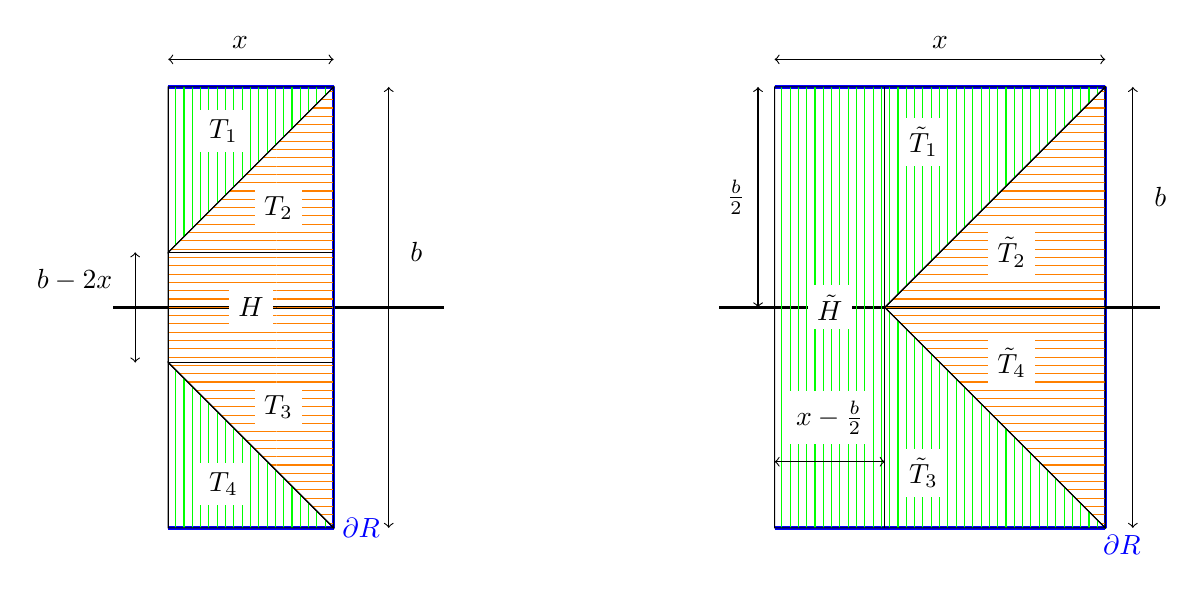
\begin{tikzpicture}[scale=0.7]
			\draw[black, very thick]
			(-12,0) -- (-6,0);
			\draw[blue,very thick] 
			(-11,-4) -- (-8,-4);
			\draw[blue,very thick] 
			(-11,4) -- (-8,4);
			\draw[blue,very thick]
			(-8,-4) -- (-8,4);
			\draw (-11,1) -- (-8,1);
			\draw (-11,-1) -- (-8,-1);
			\draw [pattern={horizontal lines}, pattern color=orange]
			(-11,1) -- (-8,4) --(-8,-4)-- (-11,-1) --cycle;
			\draw [pattern={vertical lines}, pattern color=green]
			(-11,1) -- (-11,4) --(-8,4)--cycle;
			\draw [pattern={vertical lines}, pattern color=green]
			(-11,-1) -- (-11,-4) --(-8,-4)--cycle;
			\draw [black,very thick]	
			(-10,-3.2) node[ fill=white]{$T_4 $} ;
			\draw [black,very thick]	
			(-9,-1.8) node[ fill=white]{$T_3 $} ;
			\draw [black,very thick]	
			(-10,3.2) node[ fill=white]{$T_1 $} ;
			\draw [black,very thick]	
			(-9,1.8) node[ fill=white]{$T_2 $} ;
			\draw [black,very thick]	
			(-9.5,0) node[ fill=white]{$H $} ;
			\draw [blue,very thick]	
			(-7.5,-4) node{$\partial R $} ;
			\draw [<->] (-7,-4) -- (-7,4);
			\draw
			(-6.5,1) node{$ b $} ;
			\draw [<->] (-11.6,-1) -- (-11.6,1);
			\draw
			(-12.7,0.5) node{$ b-2x $} ;
			\draw [<->] (-11,4.5) -- (-8,4.5);
			\draw
			(-9.7,4.8) node{$ x $} ;
			\draw[blue,very thick] 
			(0,-4) -- (6,-4);
			\draw[blue,very thick] 
			(6,-4) -- (6,4);
			\draw[blue,very thick]
			(0,4) -- (6,4);
			\draw[black,very thick]
			(-1,0) -- (7,0);
			\draw [pattern={horizontal lines}, pattern color=orange]
			(6,-4) -- (6,4) --(2,0) --cycle;
			\draw [pattern={vertical lines}, pattern color=green]
			(2,0)--(6,4) -- (0,4)--(0,-4) -- (6,-4)--cycle;
			\draw (2,4)--(2,-4);
			\draw [black,very thick]	
			(1,0) node[ fill=white]{$\tilde{H} $} ;
			\draw [black,very thick]	
			(2.7,3) node[ fill=white]{$\tilde{T}_1 $} ;
			\draw [black,very thick]	
			(2.7,-3) node[ fill=white]{$\tilde{T}_3 $} ;
			\draw [black,very thick]	
			(4.3,1) node[ fill=white]{$\tilde{T}_2 $} ;\draw [black,very thick]	
			(4.3,-1) node[ fill=white]{$\tilde{T}_4 $} ;
			\draw [<->] (0,4.5) -- (6,4.5);
			\draw
			(3,4.8) node{$ x $} ;
			\draw [<->] (6.5,4) -- (6.5,-4);
			\draw
			(7,2) node{$ b $} ;
			\draw [<->] (-0.3,4) -- (-0.3,0);
			\draw
			(-0.7,2) node{$ \frac{b}{2} $} ;
			\draw [<->] (0,-2.8) -- (2,-2.8);
			\draw
			(1,-2) node[ fill=white]{$ x-\frac{b}{2} $} ;
			\draw [blue,very thick]	
			(6.3,-4.3) node{$\partial R $} ;
		\end{tikzpicture}

\end{document}